\documentclass[tikz,border=4pt]{standalone}
% Shared style for every figure and for the deck: one accent, one
% highlight, thin lines, rounded nodes, nothing decorative.
\usepackage[T1]{fontenc}
\usepackage{lmodern}
\renewcommand{\familydefault}{\sfdefault}
\usepackage{tikz}
\usetikzlibrary{arrows.meta,positioning,calc,shapes.misc,fit,backgrounds,decorations.pathreplacing}
\definecolor{ink}{RGB}{40,40,40}
\definecolor{soft}{RGB}{150,150,150}
\definecolor{faint}{RGB}{225,225,225}
\definecolor{accent}{RGB}{0,95,115}
\definecolor{accentlight}{RGB}{214,232,236}
\definecolor{warn}{RGB}{196,84,40}
\definecolor{warnlight}{RGB}{247,226,216}
\tikzset{
  every picture/.style={color=ink, line width=0.5pt, font=\small},
  node distance=12mm and 18mm,
  box/.style={draw=ink, rounded corners=2pt, fill=white, inner sep=5pt, minimum height=7mm, align=center},
  maker/.style={box, minimum width=18mm},
  cat/.style={box, inner sep=3.5pt, minimum height=6mm},
  root/.style={box, fill=accentlight, draw=accent},
  bad/.style={box, fill=warnlight, draw=warn},
  ghost/.style={box, draw=soft, text=soft, dashed},
  flow/.style={-{Stealth[length=4pt,width=3.5pt]}, line width=0.5pt},
  sub/.style={-{Stealth[length=4pt,width=3.5pt]}, line width=0.5pt, color=soft},
  strong/.style={flow, color=accent, line width=0.8pt},
  wrong/.style={flow, color=warn},
  lbl/.style={font=\footnotesize, text=ink, inner sep=1.5pt, fill=white},
  note/.style={font=\footnotesize, text=soft, align=center},
  rate/.style={font=\footnotesize, text=accent, inner sep=1pt, fill=white},
}

\usepackage{amsmath}
\usepackage{pgfplots}
\pgfplotsset{compat=1.17}

\begin{document}
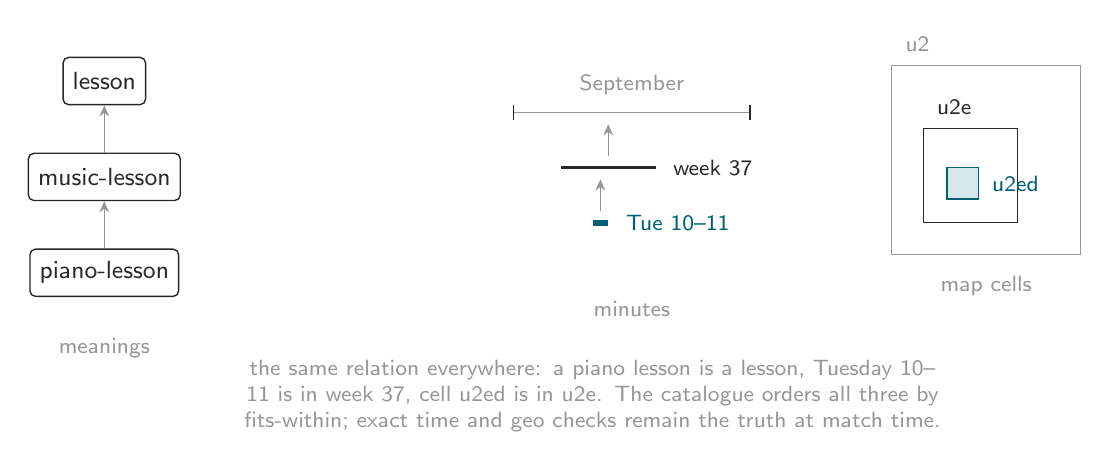
\begin{tikzpicture}
  % categories
  \begin{scope}
    \node[cat] (l) {lesson};
    \node[cat, below=6mm of l] (m) {music-lesson};
    \node[cat, below=6mm of m] (p) {piano-lesson};
    \draw[sub] (m) -- (l); \draw[sub] (p) -- (m);
    \node[note, below=4mm of p] {meanings};
  \end{scope}
  % time
  \begin{scope}[xshift=52mm, yshift=-4mm]
    \draw[soft] (0,0) -- (30mm,0);
    \draw[draw=ink] (0,1mm) -- (0,-1mm) (30mm,1mm) -- (30mm,-1mm);
    \node[note, above=1mm] at (15mm,0) {September};
    \draw[draw=ink, line width=1.2pt] (6mm,-7mm) -- (18mm,-7mm);
    \node[note, right, text=ink] at (19mm,-7mm) {week 37};
    \draw[draw=accent, line width=2pt] (10mm,-14mm) -- (12mm,-14mm);
    \node[note, right, text=accent] at (13mm,-14mm) {Tue 10--11};
    \draw[sub] (11mm,-12.5mm) -- (11mm,-8.5mm);
    \draw[sub] (12mm,-5.5mm) -- (12mm,-1.5mm);
    \node[note] at (15mm,-25mm) {minutes};
  \end{scope}
  % space
  \begin{scope}[xshift=100mm, yshift=-22mm]
    \draw[soft] (0,0) rectangle (24mm,24mm);
    \node[note, anchor=south west] at (0.5mm,24.5mm) {u2};
    \draw[ink] (4mm,4mm) rectangle (16mm,16mm);
    \node[note, anchor=south west, text=ink] at (4.5mm,16.5mm) {u2e};
    \draw[accent, fill=accentlight] (7mm,7mm) rectangle (11mm,11mm);
    \node[note, text=accent, anchor=west] at (11.5mm,9mm) {u2ed};
    \node[note] at (12mm,-4mm) {map cells};
  \end{scope}
  \node[note, text width=120mm] at (62mm,-40mm) {the same relation everywhere: a piano lesson is a lesson, Tuesday 10--11 is in week 37, cell u2ed is in u2e. The catalogue orders all three by fits-within; exact time and geo checks remain the truth at match time.};
\end{tikzpicture}
\end{document}
